\chapter{Een bibliografische databank bijhouden}%
\label{ch:bibliografie}

In het vorige hoofdstuk (zie Hoofdstuk~\ref{ch:literatuuroverzicht}) hebben we besproken hoe je gericht op zoek kan gaan naar ict-gerelateerde vakliteratuur. Het is belangrijk om alle informatie die je op die manier gevonden hebt op een gestructureerde manier bij te houden, zodat je bij het schrijven van je scriptie of paper kan verwijzen naar je bronnen en zodat je de referentielijst of bibliografie kan opmaken. Hoe je dat aanpakt kom je te weten in dit hoofdstuk.

Het verwijzen naar bronnen en opmaken van een bibliografie moet op een strakke, strikt vastgelegde manier gebeuren. Hiervoor bestaan verschillende stijlen, bv.\ de Chicago Manual of Style, IEEE, American Psychological Association (APA), enz. Op HOGENT is gekozen voor de APA-stijl\footnote{Zie cursus \emph{Kritisch Denken en Onderzoekscompetenties voor de Bachelorstudent} op Chamilo}, wellicht de belangrijkste standaard voor publicaties in het domein van de sociale wetenschappen. Het gebruik ervan is dus verplicht voor alle scripties en papers in alle opleidingen van de hogeschool. Dat geldt zowel voor de opmaak van de literatuurlijst als refereren naar bronnen in de tekst.

De opmaakregels voor referenties en bibliografieën in de APA-stijl zijn uitgebreid en vrij complex. Gelukkig hoeven we dit niet volledig manueel te doen. Er bestaan softwarepakketten die dit grotendeels automatiseren: bibliografische databanken of (in het Engels) \emph{reference management software}.

\section{Bibliografische databank}%
\label{sec:bibliografische-databank}

Een bibliografische databank laat je toe metadata over de gelezen werken gestructureerd bij te houden: titel, auteur, jaartal, en dergelijke, maar ook (aanklikbare) URLs, PDFs van artikels, nota's, enz.

In de cursus \emph{Kritisch Denken en Onderzoekscompetenties voor de Bachelorstudent} wordt gesuggereerd om Endnote te gebruiken als bibliografische databank. Het nadeel hiervan is dat dit een commerciële applicatie is, waar je na je afstuderen geen toegang meer toe hebt.

In deze sectie stellen we JabRef\footnote{\url{http://www.jabref.org/}} voor, een open source applicatie die bovendien ontwikkeld is specifiek voor {\LaTeX}. JabRef gebruikt als bestandsformaat het ingebouwde systeem voor bibliografieën, Bib{\LaTeX}. Dit is een tekstformaat met aangepaste syntax voor bibliografische gegevens. Je kan het dus in principe bewerken met een teksteditor, maar JabRef biedt een gebruiksvriendelijke interface om dit te doen en helpt bij het invullen van de correcte velden.

\subsection{JabRef}%
\label{ssec:jabref}

Je kan JabRef installeren op Windows, macOS of Linux volgens de instructies op de website, of in onze online {\LaTeX} gebruikersgids\footnote{Zie \url{https://hogenttin.github.io/latex-hogent-gids/}}.

Als je meer gedetailleerde informatie over Bib{\LaTeX} nodig hebt, die niet in deze gids te vinden is, raadpleeg dan de handleiding~\autocite{Kime2024}.

\begin{figure}
  \centering
  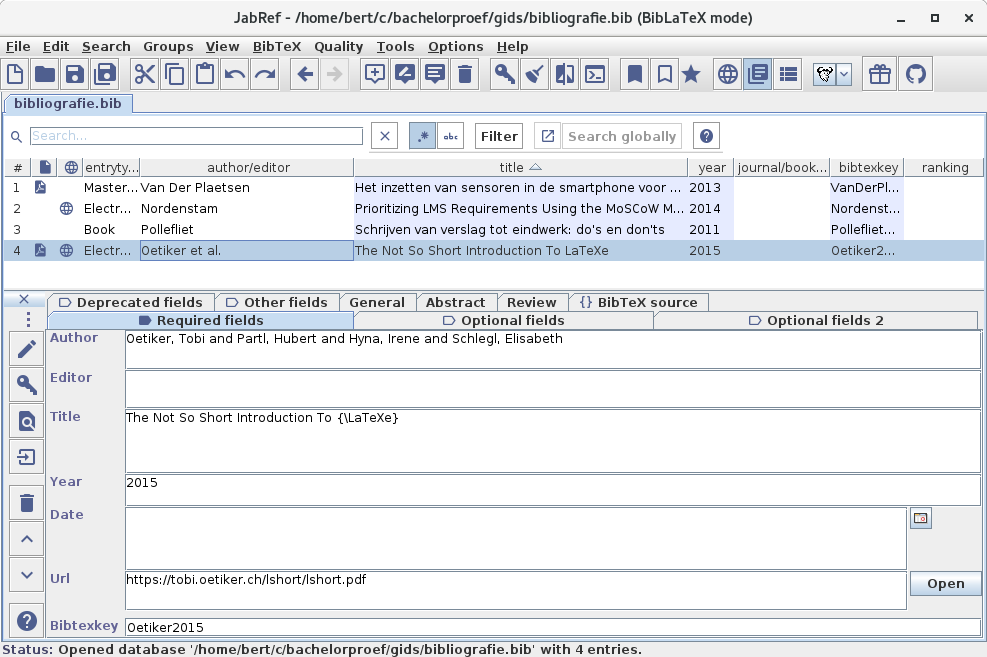
\includegraphics[width=\linewidth]{4/jabref-screenshot}
  \caption[JabRef]{\label{fig:jabref}\textbf{JabRef.} Centraal in de gebruikersinterface vind je een lijst van de verschillende bronnen in deze bibliografische databank. De pdf-icoontjes links bij de tweede en vierde bron geven aan dat de bron lokaal opgeslagen is als pdf. Als je hierop klikt, wordt de pdf geopend. De ketting-icoontjes die bij verschillende bronnen voorkomen duiden op een url die je in de webbrowser kan openen als je hierop klikt. Als je een bron selecteert, dan krijg je onderaan links invulvakken te zien met de bijgehouden metadata voor die bron. Deze worden opgedeeld in verschillende tabbladen, o.a.~verplichte gegevens (``Required fields''), optionele (``Optional'') en andere (``Other fields''), enz. In dit geval zijn de namen van de auteurs ingevuld (zie Sectie~\ref{sec:algemene_bibliografische_gegevens}). Er zijn in dit geval geen redacteurs (``Editors''), en dat veld is dan ook leeg gebleven. Het veld ``Citationkey'' onderaan is automatisch gegenereerd (zie Sectie~\ref{sub:jabref_instellingen}) door te klikken op de knop met het sleutelsymbool en label ``Generate'' rechts van het invulvak. Rechtsonder zie je een ``Preview,'' wat een idee zou moeten geven van hoe de referentie er uit zal zien in de bibliografie.}

\end{figure}

\subsection{JabRef instellingen}%
\label{sub:jabref_instellingen}

Wanneer je JabRef voor het eerst opent, is het nuttig om volgende instellingen aan te passen via Options > Preferences:

\begin{itemize}
  \item \textbf{General:} Default bibliography mode: wijzig dit naar biblatex. In de standaardinstelling (BibTeX) is er geen ondersteuning voor Unicode of voor de APA-stijl.
  \item \textbf{Entry preview:} Selecteer in de beschikbare stijlen de APA-stijl. Je krijgt dan rechtsonder in het venster een voorbeeld van de opmaak van de referentie in de APA-stijl. Dit is niet perfect, maar geeft wel een idee van hoe de bronvermelding er uit zal zien in de bibliografie.
  \item \textbf{Linked Files:} en geef een directory op voor het bijhouden van PDFs van de gevonden bronnen onder ``Main file directory''. Het is heel interessant om de gevonden artikels te downloaden en onder die directory bij te houden. Nog beter is om als naam van het bestand de BibTeX citation key te nemen (bv.\ Knuth1998.pdf). Je kan het bestand dan makkelijk openen vanuit JabRef.
\end{itemize}

Je kan de andere instellingen nakijken en eventueel naar wens aanpassen, maar de hierboven opgesomde zijn de belangrijkste.

\section{Een bibliografie invoegen in een {\LaTeX}-document}%
\label{sec:een_bibliografie_invoegen_in_een_latex_document}

Eens je enkele bronnen in een Bib{\LaTeX}-bestand hebt opgeslagen, kan je die gebruiken in je {\LaTeX}-document. In de {\LaTeX}-sjablonen voor het onderzoeksvoorstel en voor de bachelorproef zit de APA-stijl al ingebakken en je hoeft je dus helemaal geen zorgen te maken over de correcte opmaak. Dit gebeurt automatisch, mits je de bibliografische gegevens (bv.\ titel, auteur, jaar van publicatie) correct bijhoudt in Jabref.

Voor de volledigheid geven we hier de nodige instructies om dit ook in andere {\LaTeX}-documenten te kunnen toepassen.

Je hebt minstens een {\LaTeX}-bestand nodig en een Bib{\LaTeX}-bestand. In het {\LaTeX}-bestand moet je de in de ``preamble'' (d.w.z.\ vóór het \texttt{{\textbackslash}begin\{document\}} comman\-do) volgende instructies toevoegen:

\begin{minted}[frame=lines,linenos]{latex}
  \usepackage[backend=biber,style=apa]{biblatex}
  \DeclareLanguageMapping{dutch}{dutch-apa}
  \addbibresource{<naam van je BibLaTeX-bestand>.bib}
\end{minted}

De eerste regel zorgt er voor dat de APA-stijl wordt toegepast. De tweede regel zorgt er voor dat eventueel door {\LaTeX} gegenereerde tekst in het Nederlands wordt weergegeven. De derde regel zorgt er voor dat het opgegeven bibliografische databankbestand als bron kan gebruikt worden om referenties op te zoeken.

Achteraan het {\LaTeX}-bestand moet je dan de volgende instructie toevoegen:

\begin{minted}[frame=lines,linenos]{latex}
  \printbibliography
\end{minted}

Als je dit doet in een nieuw document en je compileert op dit punt, zal je wellicht merken dat er nog geen bibliografie wordt weergegeven. Dat komt omdat je nog geen referenties hebt toegevoegd. In een bibliografie mogen immers enkel werken vermeld worden waar ook effectief naar gerefereerd wordt in de tekst.

Over refereren kan je meer lezen in sectie~\ref{sec:bibliografie-refereren}.

\subsection{Wat als de bibliografie niet verschijnt?}%
\label{ssec:wat_als_de_bibliografie_niet_verschijnt}

Als je toch refereert in de tekst, maar je ziet na compileren nog steeds geen bibliografie, dan kan je volgende zaken controleren. Kijk ook naar de uitvoer van de compilatie voor foutboodschappen die je kunnen helpen bij het oplossen van het probleem.

\begin{itemize}
  \item Zijn er referenties in de tekst? \verb|\textcite| of \verb|\autocite| moet minstens één keer gebruikt worden.
  \item Misschien is bij het genereren van het PDF-document de bibliografie niet gecompileerd. In {\TeX}studio kan je dit forceren door in de menubalk te kiezen voor ``Tools > Bibliography'' (of sneltoets F8). Dan wordt \texttt{biber} uitgevoerd die alle referenties in de tekst opzoekt en het nodige doet om de bibliografie te genereren. Daarna moet je nog eens compileren (``Tools > Build \& View'' of F5) en nu zou de bibliografie moeten verschijnen.
  \item Als je in de PDF op de plaats van een referentie de ``citation key'' in het vet ziet staan, dan betekent het dat deze niet gevonden is in de bibliografische databank. Controleer of je de juiste citation key hebt gebruikt en of deze inderdaad voorkomt in het Bib{\LaTeX}-bestand.
\end{itemize} 

\section{Soorten bronnen}%
\label{sec:soorten_bronnen}

De bedoeling van een bibliografie is de lezer toelaten jouw bronnen zelf op te zoeken en te beoordelen op betrouwbaarheid. Dat betekent dat je voldoende informatie moet opgeven zodat de bron terug te vinden is. Afhankelijk van het soort bron moet je andere, specifieke informatie opgeven. Dit wordt verderop uitgediept.

Bij het toevoegen van een nieuwe bron aan een bibliografische databank moet je eerst het type selecteren (zie Afbeelding~\ref{fig:jabref-entrytypes}).

\begin{figure}
  \centering
  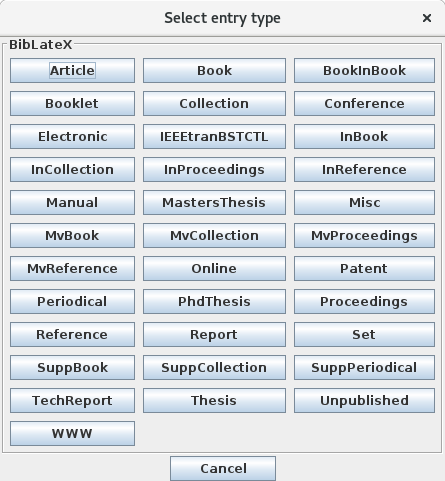
\includegraphics[width=0.6\linewidth]{4/jabref-entrytypes}
  \caption[Soorten bronnen in JabRef]{\label{fig:jabref-entrytypes}\textbf{Soorten bronnen in JabRef.} Bij het toevoegen van een nieuwe bron in JabRef (Ctrl+N) moet je eerst het soort publicatie kiezen. Afhankelijk van het soort moet in de literatuurlijst immers andere informatie gegeven worden.}
\end{figure}

Bib{\LaTeX} onderscheidt onder andere de volgende soorten bronnen:

\begin{description}
  \item[Article] Een artikel in een wetenschappelijke journal;
  \item[Online] Een online gevonden bron zoals blog-artikel van een vakexpert, video van een presentatie op een vakconferentie, artikel in een online publicatie zoals Dzone of InfoQ, enz. (synoniemen: WWW, Electronic);
  \item[Book, InBook] Een boek of hoofdstuk in een boek;
  \item[Thesis] Een scriptie of eindwerk van een student (bachelorproef, masterthesis, doctoraatsproefschrift);
  \item[Report] Een (onderzoeks-)rapport, typisch uitgegeven door een hoger onderwijsinstelling, onderzoeksgroep, overheidsinstelling, bedrijf, enz.
  \item[InProceedings] Een artikel in de ``proceedings'' van een conferentie, een boek waar\-in alle artikels gebundeld zijn die op de conferentie werden gepresenteerd;
  \item[enz.] Er zijn nog andere soorten bronnen, maar deze komen minder vaak voor of zijn niet relevant voor een bachelorproef informatica.
\end{description}

\section{Automatisch invullen van bibliografische gegevens}%
\label{sec:automatisch_invullen_van_bibliografische_gegevens}

Sommige tertiaire bronnen zoals ScienceDirect, Springer, Google Scholar, enz.\ bieden de mogelijkheid om de nodige informatie automatisch in te vullen. Dat kan op verschillende manieren.

Op de webpagina voor het gevonden artikel kan je de bibliografische gegevens in Bib{\LaTeX}-formaat kopiëren of downloaden. Zoek naar een link of knop met de vermelding ``Cite'', klik er op door en selecteer Bib{\LaTeX}. Kopieer de tekst en plak die in JabRef via het tabblad ``biblatex source''.

Een andere manier is via een unieke code die de bron identificeert. Voor boeken is dat het ISBN-nummer. Als je een nieuwe bron toevoegt (zie Figuur~\ref{fig:jabref-entrytypes}), kan je in het drop-down veld ``ID type'' ISBN kiezen en het nummer erin plakken. Klik vervolgens op ``Generate'' en de belangrijkste velden worden (in principe) meteen ingevuld.

Voor artikels die in journals gepubliceerd zijn, is er een gelijkaardig systeem: Ditigal Object Identifier of DOI. Dit is een unieke code die je kan vinden op de webpagina van het artikel. De vorm is meestal:

\begin{center}
  \texttt{https://doi.org/UITGEVER/ARTIKEL}

  bv. \texttt{https://doi.org/10.1016/j.ijinfomgt.2015.11.010}
\end{center}

Elke uitgever heeft een eigen code (bv. 10.1016 voor Elsevier, 10.1007 voor Springer, enz.) en binnen hun publicaties geven zij ook elk individueel artikel een ID. Bij het toevoegen van een nieuwe bron kies je als ``ID type'' voor DOI en kopieer en plak je het \texttt{UITGEVER/ARTIKEL}-gedeelte van de DOI-url (dus zonder \texttt{https://doi.org/}) in het invulveld.

Ook de documentatie over de TCP/IP-protocolstack kan je op deze manier toevoegen. Deze zijn online gepubliceerd\footnote{Zie \url{https://www.rfc-editor.org}} in de vorm van zgn.~RFC's (Request for Comment). Je kan als ``ID Type'' voor RFC kiezen en dan het nummer van de RFC invullen.

Merk op dat deze systemen niet altijd perfect werken, dus controleer altijd het resultaat! En misschien wil je nog informatie toevoegen die niet werd ingevuld via de ID, bv.\ de abstract, sleutelwoorden, enz.


\section{Algemene bibliografische gegevens}%
\label{sec:algemene_bibliografische_gegevens}

 Drie elementen zijn sowieso \emph{altijd} essentieel: de \textbf{auteur}, de \textbf{titel} van de bron en het \textbf{datum} (of tenminste het jaar) van publicatie. Als één van deze drie ontbreekt, wordt het bijzonder moeilijk om de oorsprong en de kwaliteit van de bron te evalueren. Dit soort bronnen kan je bijhouden ter info, maar zijn meestal niet geschikt om op te nemen in een bibliografie. Als de auteur onbekend is, is het immers niet mogelijk om te beoordelen of die wel de autoriteit heeft om op een objectieve en diepgaande manier over het onderwerp te schrijven. Als het jaartal niet opgegeven is, is het erg moeilijk om na te gaan in hoeverre deze bron nog niet achterhaald is door recentere ontwikkelingen in het vakgebied.

\subsection{Het Author-veld}%
\label{ssec:het_author_veld}

Enkele tips bij het invullen van auteursnamen:

\begin{itemize}
  \item Noteer de naam van auteurs in de vorm ``Familienaam, Voorna(a)m(en)''. Dus ``Van Vreckem, Bert'' en niet ``Bert Van Vreckem.'' In principe wordt de tweede notatie ook aanvaard, maar dit werkt enkel voor typische angelsaksische namen met een tweede voornaam (bv. ``Donald Ervin Knuth''). De eerste twee woorden worden beschouwd als voornamen, het laatste woord als de familienaam. ``Van'' wordt in dat geval dus verkeerdelijk beschouwd als tweede voornaam.
  \item Als de auteur een bedrijf of organisatie is, met een naam bestaande uit verschillende woorden, zet die dan tussen accolades: bv. ``\{The Linux Foundation\}''. Zoniet probeert {\LaTeX} dit als een persoonsnaam te interpreteren. ``Foundation'' wordt dan de familienaam, ``The'' en ``Linux'' de twee voornamen.
  \item Als je meerdere auteurs hebt, scheid elke naam dan met \texttt{and}, bv. ``Bernard, Anita and Buysse, Jens and Van Vreckem, Bert''.
  \item Na invullen van de auteursna(a)m(en) klik je op de knop met het sleutel-icoon (zie Figuur~\ref{fig:jabref}) om een unieke sleutel te genereren voor deze bron.
  \item Naast een auteurveld is er ook een veld voor eventuele redacteur(s) (\emph{editor}) voorzien. Minstens één van beide moet ingevuld zijn, soms allebei. Dit gebeurt bijvoorbeeld in een boek dat samengesteld is uit hoofdstukken die telkens door andere auteurs geschreven zijn en waar je naar één bepaald hoofdstuk wil verwijzen. Verderop vind je daar een voorbeeld van.
\end{itemize}

\subsection{Het Date-veld}%
\label{ssec:het_date_veld}

Data worden in Bib{\LaTeX} altijd in het formaat \texttt{jjjj-mm-dd} ingegeven (volgens de ISO-8601 standaard), dus eerst het jaar, dan de maand en tenslotte de dag, gescheiden met koppeltekens (-).

Als je de maand of de dag niet kent, vernoem je enkel het jaar.

Bij het importeren van bibliografische gegevens wordt soms niet het Date-veld ingevuld, maar Year. Dit is een overblijfsel van de Bib{\TeX} standaard, waar er aparte velden voorzien waren voor het jaartal (Year) en maand (Month, weergegeven door de eerste drie letters van de maand in het Engels: Jan, Feb, Mar, enz.).

Je kan de inhoud van het Year-veld (en desgevallend Month) het best naar Date kopiëren.

\subsection{Extra informatie bijhouden}%
\label{ssec:extra_informatie_bijhouden}

Probeer telkens zoveel mogelijk informatie bij te houden over je bronnen, zodat het later makkelijker wordt die terug te vinden. Dit is een tijdrovend proces, en niet al deze informatie wordt ook in de bibliografie opgenomen. Het raadplegen van de databank wordt wel een stuk makkelijker.

Enkele velden die zinvol zijn om altijd trachten in te vullen, ook al zijn ze niet verplicht en worden ze ook niet altijd in de bibliografie getoond:

\begin{description}
  \item[Abstract] Samenvatting van het artikel. Dit is meestal de eerste paragraaf van een artikel en wordt altijd duidelijk aangegeven.
  \item[DOI] of ``Digital Object Identifier''. Dit is een unieke code voor artikels in wetenschappelijke publicaties die het opzoeken makkelijker maakt (op voorwaarde dat de DOI gegeven is).
  \item[File] Naam van het bestand met het gedownloade artikel. Je kan vanuit JabRef het artikel openen in een PDF-viewer of desgevallend tekstverwerker.
  \item[Keywords] Kernwoorden i.v.m~het onderwerp, gescheiden door komma's.
  \item[Review] Je eigen opmerkingen over deze bron. Waarom heb je deze bijgehouden? Wat is het interessantste dat je er uit geleerd hebt?
  \item[URL] De URL waar je het artikel gevonden hebt. Deze URL wordt niet altijd in de bibliografie opgenomen, maar is altijd nuttig om bij te houden. Je kan vanuit JabRef de website openen in een webbrowser.
  \item[Urldate] de datum waarop je deze bron het laatst hebt geraadpleegd.
\end{description}

Let er tenslotte ook op dat je in Jabref \textbf{nooit speciale lettertekens gebruikt} die voor {\LaTeX} een specifieke betekenis hebben. Het gaat hier dan onder andere over het percentteken (\%), het hekje (\#), het dollarteken (\$), het ampersand-teken (\&) en de accolades (\{ en \}). Als je deze toch nodig hebt, moet je er meestal een backslash voor zetten, bv. ``\textbackslash\%'' of het geschikte commando voor dat specifieke teken gebruiken. Als je dit over het hoofd ziet, zal je compilatie mislukken en jammer genoeg is de foutboodschap vaak niet erg duidelijk.

\section{Specifieke bibliografische gegevens}%
\label{sec:specifieke_bibliografische_gegevens}

In deze sectie wordt voor de meest relevante soorten bronnen uitgelegd hoe deze correct bij te houden en in de bibliografie op te nemen. JabRef geeft zelf al enige aanwijzingen over welke informatie minstens nodig is: in het detailvenster (zie Afbeelding~\ref{fig:jabref}) moet je minstens het tabblad ``Required fields'' invullen. Voor elk soort publicatie (zie Sectie~\ref{sub:publicatievormen}) vind je verderop een overzicht van de in te vullen velden en wat die precies betekenen, en hoe de referentie in de literatuurlijst er uit zal zien.

\subsection{Article}%
\label{ssec:article}

Dit soort bron wordt enkel gebruikt voor artikels die verschenen zijn in een wetenschappelijke journal. Artikels in (vak)tijdschriften of kranten vallen hier \emph{niet} onder, maar daarvoor gebruik je het type Periodical.

Verplichte velden voor Article:

\begin{description}
  \item[Author] De naam van de auteur;
  \item[Title] De titel van het artikel;
  \item[Journaltitle] De naam van het tijdschrift;
  \item[Date] Verschijningsdatum (of -jaar) van het artikel;
  \item[Volume] De jaargang van het tijdschrift waarin het artikel verschenen is;
  \item[Number] Het nummer (binnen de jaargang) waarin het artikel verschenen is (soms niet gegeven);
  \item[Pages] Paginanummers
\end{description}

Voorbeeld broncode:
\begin{minted}[frame=lines,linenos,breaklines]{bibtex}
@Article{SabiEtAl2016,
  author       = {Sabi, Humphrey M. and Uzoka, Faith-Michael E. and Langmia, Kehbuma and Njeh, Felix M.},
  title        = {Conceptualizing a model for adoption of cloud computing in education},
  journaltitle = {International Journal of Information Management},
  date         = {2016},
  volume       = {36},
  number       = {2},
  pages        = {183--191},
  doi          = {10.1016/j.ijinfomgt.2015.11.010},
  url          = {http://www.sciencedirect.com/[...]8401215001115},
  abstract     = {Cloud computing is a pervasive computing [...]},
  keywords     = {Cloud computing, Educational technologies, [...]},
}
\end{minted}

In de bibliografie ziet dit er zo uit: \fullcitebib{SabiEtAl2016}

\subsection{Online}%
\label{ssec:online}

Onder dit type publicatie vallen vrijwel alle online bronnen die niet onder een andere categorie te plaatsen zijn: blogartikels, artikels in online vaktijdschriften of portaalsites, Youtube-video's van presentaties op vakconferenties, online documentatie, enz.

Merk op dat je de algemene website van organisaties, softwarepakketten, enz. \emph{niet} in je literatuurlijst mag opnemen. Deze kan je wel in een voetnoot zetten.

Deze velden moet je verplicht invullen:

\begin{description}
  \item[Author] Auteur(s) van de bron, spreker (in het geval van een video van een lezing op een conferentie), \ldots
  \item[Title] Titel van de bron, lezing, \ldots
  \item[Date] Datum (of jaar) van publicatie,
  \item[URL] naar de website waar de bron kan teruggevonden worden,
  \item[Urldate] Datum van laatste raadplegen,
\end{description}

Bij dit soort bronnen worden veel fouten gemaakt bij het refereren. Het is essentieel dat de URL wordt meegegeven en ook de datum van raadplegen. Het web is voortdurend in beweging, en het is mogelijk dat de inhoud van een webpagina in de loop van de tijd verandert (bv.\ fouten die verbeterd worden) of zelfs dat een website herstructureert en de URL dus op een gegeven manier niet meer geldig is. Door de datum van raadplegen op te geven, bied je de lezer nog de kans om terug te vinden hoe die website er op dat moment in de tijd uitzag, via bijvoorbeeld de Wayback Machine van het Internet Archive\footnote{\url{https://archive.org/web/}}.

Vergeet niet om de URL goed na te kijken en overbodige informatie te verwijderen, zoals:

\begin{itemize}
  \item \texttt{\&utm\_source=\ldots}, parameters in de URL die gebruikt worden om de herkomst van de bezoeker te traceren. Deze zijn niet nodig om de pagina terug te vinden.
  \item \texttt{\#:\textasciitilde:text=Highlighted\%20text}, code die bepaalde tekst op de pagina markeert.
\end{itemize}

Voorbeeld van een blogartikel:

\begin{minted}[frame=lines,linenos,breaklines]{bibtex}
@Online{LewisFowler2014,
  author    = {Lewis, James and Fowler, Martin},
  title     = {Microservices: a definition of this new architectural term},
  date      = {2014-03-25},
  url       = {http://martinfowler.com/articles/microservices.html},
  urldate   = {2016-09-01},
  abstract  = {The term "Microservice Architecture" has [...]},
  keywords  = {application architecture, web services, microservices},
}
\end{minted}

In de bibliografie wordt dit: \fullcitebib{LewisFowler2014}

Een ander voorbeeld, deze keer van een presentatie op een vakconferentie die op Youtube is gepubliceerd. Omdat er niet meteen een apart veld voorzien is voor het vermelden van de naam van de conferentie, is die hier in het titelveld verwerkt.

\begin{minted}[frame=lines,linenos,breaklines]{bibtex}
@Online{Hykes2013,
  author       = {Solomon Hykes},
  title        = {The future of Linux Containers (PyCon 2013)},
  date         = {2013-03-21},
  url          = {https://www.youtube.com/watch?v=wW9CAH9nSLs},
  urldate      = {2016-09-01},
  abstract     = {At PyCon Solomon Hykes shows docker to the public for the first time.},
}
\end{minted}

In de bibliografie: \fullcitebib{Hykes2013}

\subsection{Book}%
\label{ssec:book}

Dit type gebruik je voor (e-)boeken die ``officieel'' uitgegeven zijn en dus een ISBN-nummer hebben.

Minstens volgende velden moeten dan ingevuld zijn:

\begin{description}
  \item[Author] De auteur(s) van het boek,
  \item[Date] Jaartal waarin het boek werd uitgegeven,
  \item[Title] Titel van het boek,
  \item[Publisher] Naam van de uitgeverij.
\end{description}

Optioneel kan je ook volgende informatie aanvullen:

\begin{description}
  \item[Subtitle] ondertitel van het boek,
  \item[Edition] Nummer van de uitgave of druk,
  \item[Location] Stad waar de uitgeverij gevestigd is,
  \item[ISBN] Het ISBN-nummer van het boek (ter info, wordt nooit getoond in de bibliografie),
  \item[URL] Naar de pagina over het boek op de website van de uitgeverij. \textbf{Let op!} Dit is \emph{niet} de URL van een webshop waar je het boek kan kopen, noch een link naar Google Books en zeker niet naar een illegale downloadsite!
\end{description}

Voorbeeld:
\begin{minted}[frame=lines,linenos,breaklines]{bibtex}
@Book{Aitchison2011,
  author    = {Aitchison, Ron},
  date      = {2011},
  title     = {Pro DNS and BIND 10},
  isbn      = {9781430230489},
  publisher = {Apress},
}
\end{minted}

In de bibliografie:
\fullcitebib{Aitchison2011}

\subsection{InBook}%
\label{ssec:inbook}

Dit type gebruik je als je wil verwijzen naar een specifiek hoofdstuk in een boek. Minstens volgende velden moeten dan ingevuld zijn:

\begin{description}
  \item[Author] De auteur(s) van het hoofdstuk,
  \item[Editor] De redacteur(s) van het boek (indien van toepassing),
  \item[Date] Jaartal waarin het boek werd uitgegeven,
  \item[Title] Titel van het \emph{hoofdstuk},
  \item[Pages] Begin- en eindpagina van het hoofdstuk,
  \item[Booktitle] Titel van het \emph{boek},
  \item[Publisher] Naam van de uitgeverij.
\end{description}

Optioneel kan je ook volgende informatie aanvullen:

\begin{description}
  \item[Subtitle of Booksubtitle] ondertitel van het hoofdstuk of boek, resp.,
  \item[Edition] Nummer van de uitgave of druk,
  \item[Location] Stad waar de uitgeverij gevestigd is,
  \item[ISBN] Het ISBN-nummer van het boek (ter info, wordt nooit getoond in de bibliografie).
\end{description}

Bij een boek is het ongebruikelijk om een URL op te geven. Als je bijvoorbeeld ter info voor jezelf de URL van het boek op de website van de uitgever wil bijhouden, doe je dit best in een ander veld, bv. Comment of Review.

Voorbeeld
\begin{minted}[frame=lines,linenos,breaklines]{bibtex}
@InBook{Meyr2008,
  author       = {Meyr, Herbert},
  title        = {Forecast Methods},
  booktitle    = {Supply Chain Management and Advanced Planning},
  date         = {2008},
  editor       = {Stadtler, Hartmut and Kilger, Christoph},
  booksubtitle = {Concepts, Models, Software, and Case Studies},
  edition      = {4e editie},
  publisher    = {Springer},
  location     = {Heidelberg},
  isbn         = {978-3-540-24814-9},
  pages        = {461--472},
  comment      = {https://www.springer.com/us/book/9783540248149},
}
\end{minted}

In de bibliografie ziet dit er zo uit:
\fullcitebib{Meyr2008}

\subsection{Thesis}%
\label{ssec:thesis}

Onder dit type publicatie vallen doctoraatsproefschriften, masterthesissen en bachelorproeven. Dit zijn de in te vullen velden:

\begin{description}
  \item[Author] De auteur van de thesis (student of doctorandus),
  \item[Title] Titel van de scriptie
  \item[Date] Jaar of datum van indienen
  \item[Type] Soort scriptie: Bachelorproef, masterthesis, doctoraatsthesis, \ldots
  \item[Institution] Naam van de hogeschool of universiteit waar de thesis werd ingediend
\end{description}

Voorbeeld:
\begin{minted}[frame=lines,linenos,breaklines]{bibtex}
  @Thesis{VanDerPlaetsen2013,
  author      = {Van Der Plaetsen, Thomas},
  date        = {2013},
  institution = {Hogeschool Gent},
  title       = {Het inzetten van sensoren in de smartphone voor het
                 verbeteren van de fanbeleving},
  type        = {Bachelorproef},
}
\end{minted}

Resultaat in de bibliografie:
\fullcitebib{VanDerPlaetsen2013}

\subsection{Report}%
\label{ssec:report}

Onder Report vallen onderzoeksrapporten uitgegeven door onderzoeksgroepen van universiteiten of hogescholen, overheidsinstellingen of bedrijven.

Verplichte velden:

\begin{description}
  \item[Author] De auteur(s)
  \item[Date] Datum of jaar van publicatie
  \item[Title] Titel van het onderzoeksrapport
  \item[Type] Het soort rapport. In JabRef is er een dropdown-menu met de meest voorkomende types. Meestal vul je hier \texttt{resreport} in, de afkorting van ``research report''.
  \item[Institution] Instelling die het rapport uitgegeven heeft
\end{description}

Optionele velden:

\begin{description}
  \item[Subtitle] Ondertitel van het rapport
  \item[URL] URL waar de instelling het rapport gepubliceerd heeft
  \item[Urldate] Datum waarop je het rapport geraadpleegd hebt
\end{description}

Voorbeeld:
\begin{minted}[frame=lines,linenos,breaklines]{bibtex}
@Report{DeMarez2022,
  author      = {De Marez, Lieven and Sevenhant, Robbe and ...},
  date        = {2022},
  institution = {imec},
  title       = {imec.digimeter 2022},
  type        = {resreport},
  subtitle    = {Digitale trends in Vlaanderen},
  url         = {https://www.imec.be/nl/...},
  urldate     = {2023-05-01},
}
\end{minted}

Resultaat in de bibliografie:
\fullcitebib{DeMarez2022}

\subsection{InProceedings}%
\label{ssec:inproceedings}

Dit soort bron wordt gebruikt voor artikels die gepubliceerd zijn in het verslag (proceedings) van een \emph{wetenschappelijke} conferentie. Verplichte velden:

\begin{description}
  \item[Author] Naam van de auteur(s),
  \item[Title] Titel van het artikel,
  \item[Booktitle] De naam van de conferentie,
  \item[Date] Datum (of jaar) waarin de conferentie doorging.
\end{description}

Daarnaast kan je optioneel ook volgende velden invullen:

\begin{description}
  \item[URL] naar de website van de conferentie waar het artikel kan gevonden (eventueel rechtstreeks naar de pdf);
  \item[Urldate] datum waarop je deze bron het laatst geraadpleegd hebt.
  \item[DOI] op voorwaarde dat er één toegewezen is aan dit artikel.
\end{description}

Voorbeeld:
\begin{minted}[frame=lines,linenos,breaklines]{bibtex}
@InProceedings{VanVreckemEtAl2013,
  author    = {Van Vreckem, Bert and Borodin, Dmitriy and De Bruyn, Wim and Now\'{e}, Ann},
  title     = {A Reinforcement Learning Approach to Solving Hybrid Flexible Flowline Scheduling Problems},
  booktitle = {Multidisciplinary International Scheduling Conference (MISTA) 2013},
  date      = {2013},
  url       = {https://expertise.hogent.be/files/.../hffsp_la.pdf},
  urldate   = {2016-09-01},
  abstract  = {In this paper, we present a method based on Learning Automata to solve Hybrid Flexible Flowline Scheduling  Problems [...].},
}
\end{minted}

In de bibliografie ziet dit er zo uit: \fullcitebib{VanVreckemEtAl2013}

\subsection{Andere}%
\label{ssec:andere}

In JabRef zijn nog andere soorten bronnen gedefinieerd, maar deze zijn minder relevant voor een eindwerk of paper (bv. Legislation, Patent, \ldots) of komen overeen met een van de hierboven opgesomde types.

Electronic en WWW zijn bijvoorbeeld synoniemen voor Online.

Handleidingen vallen onder het type Manual, dat je kan invullen volgens de regels van een Book (als deze in boekvorm uitgegeven is), of als een Online bron (als deze online beschikbaar is).

\section{Refereren in de tekst}%
\label{sec:bibliografie-refereren}

Als je na het opvullen van je bibliografische databank met bronnen het {\LaTeX}-do\-cu\-ment zou compileren, zal je waarschijnlijk merken dat al deze nieuwe bronnen niet zichtbaar zijn in de bibliografie. Dit komt omdat in een bibliografie \textbf{enkel werken mogen opgenomen zijn waarnaar verwezen wordt vanuit de tekst}. {\LaTeX} doet dit standaard automatisch, dus als je bronnen in de lijst mist, dan betekent dit dat je die niet in de tekst gebruikt hebt.

Voor het refereren naar bronnen in de tekst zijn er twee commando's gangbaar: \texttt{{\textbackslash}textcite} en \texttt{{\textbackslash}autocite}. Het eerste commando geeft een narratieve referentie, het tweede commando geeft een referentie tussen haakjes. Het is gebruikelijk om het eerste commando te gebruiken als je de naam van de auteur(s) in de tekst vermeldt, en het tweede commando als je de naam van de auteur(s) niet in de tekst vermeldt.

\subsection{Narratieve referenties}%
\label{ssec:narratieve_referenties}

Een voorbeeld van een narratieve referentie:

\begin{verbatim}
An overview is provided in the survey by~\textcite{RibasEtAl2010}.
For a real-life case-study of applying genetic algorithm ``on top''
of a Mixed Integer Linear Programming model, we refer
to~\textcite{BorodinEtAl2011}.
\end{verbatim}

wat resulteert in:

\begin{quotation}
  An overview is provided in the survey by Ribas, et al. (2010). For a real-life case-study of applying genetic algorithm ``on top'' of a Mixed Integer Linear Programming model, we refer to Borodin, et al. (2011).
\end{quotation}

\subsection{Referenties tussen haakjes}%
\label{ssec:referenties_tussen_haakjes}

Referenties tussen haakjes gebruik je als je de naam van de auteur(s) niet in de tekst vermeldt, bijvoorbeeld als je vakterm definieert, bij een letterlijk citaat of parafrasering of in het bijschrift van een figuur die je overgenomen hebt uit een bron.

\begin{verbatim}
Reinforcement Learning (RL) is a technique that allows an agent
to learn how to maximize a numerical reward
signal~\autocite{SuttonBarto1998}.
\end{verbatim}

wat resulteert in:

\begin{quotation}
  Reinforcement Learning (RL) is a technique that allows an agent to learn how to maximize a numerical reward signal (Sutton \& Barto, 1998).
\end{quotation}

\section{Controle}%
\label{sec:bibliografie-controle}

Het is belangrijk om na het genereren van de PDF met je finale paper of eindwerk nog eens goed te controleren of de referenties en bibliografie correct opgemaakt zijn.

\begin{itemize}
  \item Zijn de namen van de auteurs correct weergegeven? Indien de auteur een bedrijf of organisatie is, is de naam volledig weergegeven of geïnterpreteerd als een persoonsnaam?
  \item Controleer dat er geen titels VOLLEDIG IN HOOFDLETTERS staan en zet deze zo nodig om.
  \item Is er een minstens een jaartal opgegeven? Controleer ook dat nergens nog het Year- of Month-veld ingevuld is en dat de inhoud naar Date verhuisd is.
  \item Zijn de URLs correct weergegeven? Zijn er geen parameters of tracking codes in de URL geslopen?
  \item Hebben Online-bronnen ook een datum van raadplegen?
  \end{itemize}

\section{Samenvatting}%
\label{sec:bibliografie-samenvatting}

Het bijhouden van al je bronnen is tijdrovend, maar essentieel voor een goed onderbouwde bachelorproef! Besteed hier dus de nodige aandacht aan.

\begin{itemize}
  \item Zet je bibliografische databank op (bv.\ met JabRef) voordat je op zoek gaat naar informatie over je onderwerp en hou van wat je vindt nauwgezet zoveel mogelijk informatie bij.
  \item Zorg dat je altijd minstens de auteur, titel en jaartal hebt en daarnaast minstens alle andere verplichte informatie voor dat type publicatie correct noteert.
  \item Selecteer het correcte type publicatie en zorg dat in elk geval de verplichte gegevens telkens ingevuld zijn.
  \item Vergeet niet het resultaat te controleren en zo nodig aan te passen.
\end{itemize}
